\documentclass{article}
\usepackage{graphicx} % Required for inserting images
\usepackage[utf8]{inputenc}
\usepackage[T1]{fontenc}
\usepackage{karnaugh-map}
\usepackage[polish]{babel}
\usepackage{subcaption}



\begin{document}
	\begin{center}
	%\includegraphics[scale=0.35]{logo.png}	
	
	\textbf{Sprawozdanie z Laboratorium} \\
	\vspace{0.1cm}\
	\textbf{Modułowe systemy cyfrowe}
	\vspace{0.1cm}\
	\end{center}	

\noindent Wykonujący ćwiczenie: Kamil Kubajewski, Bartosz Orłowski, Jakub Matusiewicz \\
\vspace{3cm} \\
Studia dzienne I stopnia \\
Kierunek: Informatyka \\
Semestr: II \hspace{4cm} Grupa zajęciowa: LAb 8 \\
\\
Prowadzący ćwiczenie: \textbf{...} \\
\phantom{a} \hfill .................. \\
\phantom{a} \hfill OCENA \\
\\ 
\vfill \noindent
Data wykonania ćwiczenia \\
15 października 2025 r.\ \\
\phantom{a} \hfill ............................................\\
\phantom{a} \hfill Data i podpis prowadzącego

\pagebreak
\begin{center}
    \hspace{-1.2cm}
    \begin{tabular}{|p{0.7\textwidth}|l|}
        \hline
        Wydział Informatyki Politechniki Białostockiej \hfill & Data: 15.10.2025 \\
        Przedmiot: Modułowe systemy cyfrowe \hfill & \\
        \hline
        Zajęcia nr 2 & Prowadzący: \\
        Temat: Parametry statyczne i dynamiczne bramek oraz przerzutników & \textbf{...}\phantom{Phantom Phantomphantom} \\
        & \\
        Grupa: Lab 8 & \\
        Imię i nazwisko: & \\
        Kamil Kubajewski, Bartosz Orłowski, Jakub Matusiewicz & \\
        \hline
    \end{tabular}
\end{center}

\section{Cel ćwiczeń}

Zapoznanie z podstawowymi parametrami wybranych układów cyfrowych TTL, konkretnie z przerzutnikami \textbf{ D, T, RS} oraz \textbf{JK}.

\section{Podstawa teoretyczna}
Opisać teorie, m. in. napiecie +5V jako 1 i 0V jako 0, opisać zakres działania z błedem/zakresem ok. 0.7V (sprawdzic skrypt), dobrze by było dodac wykres który to przedstawia :)

\pagebreak
\section{przebieg ćwiczeń}
\subsection{Zadanie 1}
W układzie jak na rysunku zdjąć powierzchnię charakterystyczną bramki 7400. Układ
scalony 7400 umieścić w podstawce modułu DB26.

\begin{figure}[h]
    \centering
    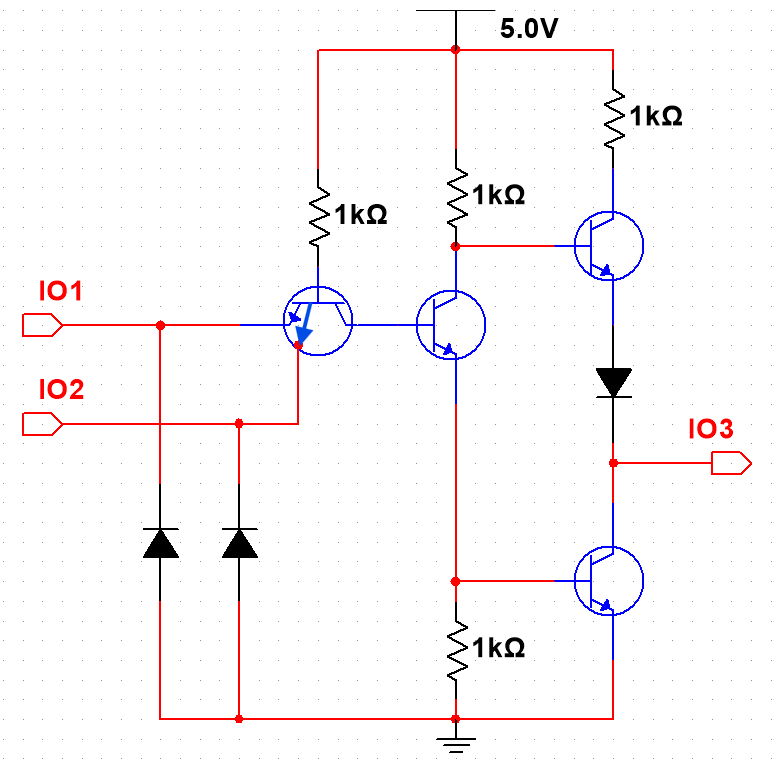
\includegraphics[width=0.8\textwidth]{obwod1.PNG}
    \caption{Bramka NAND}
    \label{fig:moj_obrazek}
\end{figure}
%\textbf{modułu DB11} przerzutniki

Do przetestowania i dokonania pomiarów użyto \textbf{modułu DB26} do którego wpięto \textbf{układ scalony 7400}, czyli bramka \textbf{NAND}. Do pomiarów dla wejśc podłączono zasilanie (5 V jako jedynka logiczna i 0 V jako zero logiczne), które było regulowane, sprawdzić otrzymane napięcie na wyjściu. Daje to poniższe pomiary(tabela 1):
\pagebreak
\begin{table}[!ht]
    \centering
    \caption{Pomiary dla rożnych danych wejść}
    \begin{tabular}{|l|l|l|}
    \hline
        V\_1 [V] & V\_2 [V] & Output[V] \\ \hline
        5,00 & 5,00 & 0,0645 \\ \hline
        4,50 & 5,00 & 0,0645 \\ \hline
        4,00 & 5,00 & 0,0645 \\ \hline
        3,50 & 5,00 & 0,0645 \\ \hline
        3,00 & 5,00 & 0,0645 \\ \hline
        2,50 & 5,00 & 0,0645 \\ \hline
        2,00 & 5,00 & 0,0645 \\ \hline
        1,50 & 5,00 & 0,0645 \\ \hline
        1,00 & 5,00 & 2,5410 \\ \hline
        0,50 & 5,00 & 3,7430 \\ \hline
        0,30 & 5,00 & 3,9290 \\ \hline
        5,00 & 4,50 & 0,0645 \\ \hline
        5,00 & 4,00 & 0,0645 \\ \hline
        5,00 & 3,50 & 0,0645 \\ \hline
        5,00 & 3,00 & 0,0645 \\ \hline
        5,00 & 2,50 & 0,0645 \\ \hline
        5,00 & 2,00 & 0,0645 \\ \hline
        5,00 & 1,50 & 0,0645 \\ \hline
        5,00 & 1,00 & 3,1890 \\ \hline
        5,00 & 0,50 & 3,9060 \\ \hline
        5,00 & 0,30 & 3,9320 \\ \hline
        1,20 & 3,70 & 2,5800 \\ \hline
        3,70 & 1,20 & 2,5500 \\ \hline
        3,10 & 0,80 & 3,4050 \\ \hline
        0,80 & 3,10 & 3,5010 \\ \hline
        1,20 & 2,80 & 2,4110 \\ \hline
        2,80 & 1,20 & 2,5620 \\ \hline
        2,80 & 2,40 & 0,0647 \\ \hline
        2,40 & 2,80 & 0,0647 \\ \hline
        1,60 & 1,20 & 2,7020 \\ \hline
        1,20 & 1,60 & 2,5330 \\ \hline
    \end{tabular}
\end{table}
\pagebreak

\begin{figure}[h]
    \centering
    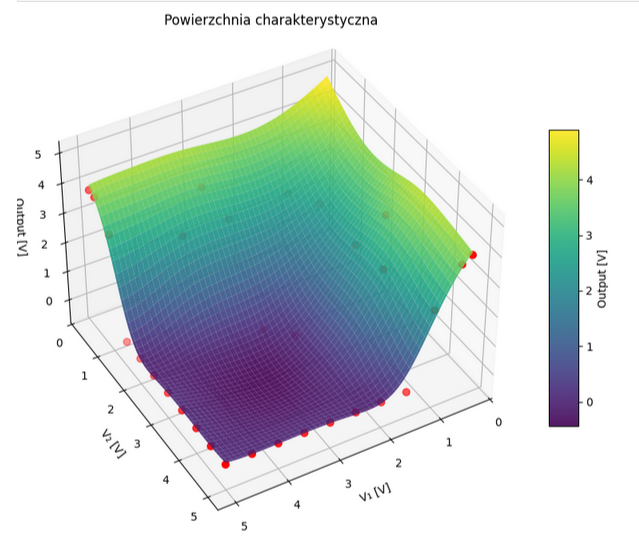
\includegraphics[width=0.5\textwidth]{powierzchnia.PNG}
    \caption{Wykres powierzchni charakterystycznej}
    \label{fig:moj_obrazek}
\end{figure}

\subsection{Zadanie 3}
W zadaniu 3 przetestowano działanie przerzutników \textbf{T, RS, JK, D} za pomocą \textbf{modułu DB11}. Poniżej zamieszczone są schematy poszczególnych przerzutników.

\begin{figure}[h]
    \centering
    \begin{subfigure}[t]{0.3\textwidth}
        \centering
        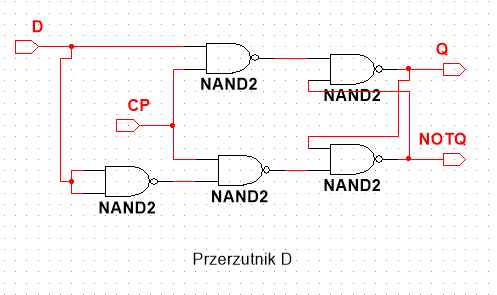
\includegraphics[width=\textwidth]{D.png}
        \caption{Schemat przerzutnika D}
    \end{subfigure}
    \hfill
    \begin{subfigure}[t]{0.3\textwidth}
        \centering
        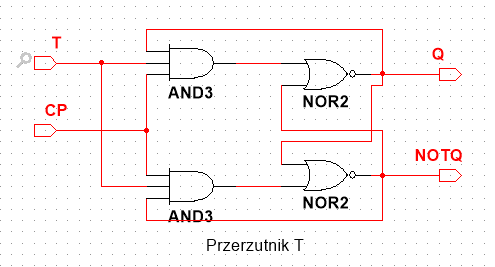
\includegraphics[width=\textwidth]{T.png}
        \caption{Schemat przerzutnika T}
    \end{subfigure}
    \hfill
    \begin{subfigure}[t]{0.3\textwidth}
        \centering
        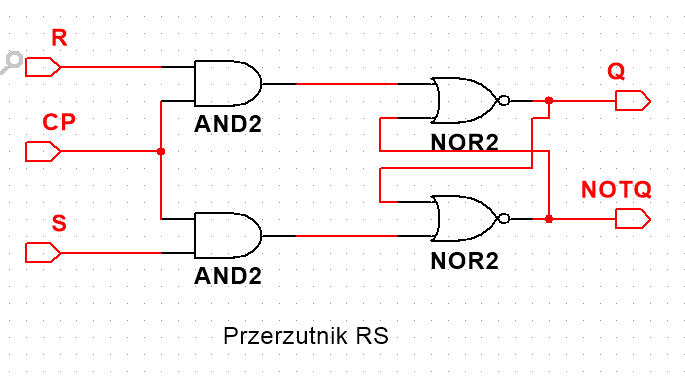
\includegraphics[width=\textwidth]{RS.png}
        \caption{Schemat przerzutnika RS}
    \end{subfigure}
        \hfill
    \begin{subfigure}[t]{0.3\textwidth}
        \centering
        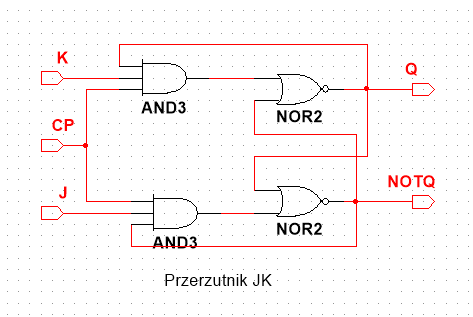
\includegraphics[width=\textwidth]{JK.png}
        \caption{Schemat przerzutnika JK}
    \end{subfigure}
    \caption{Schematy przerzutników JK, RS, T, D}
    \label{fig:bramki}
\end{figure}

\pagebreak
\section{Dyskusja błedów}
%Klasyczna formułka np. z EDI, jaka powinna byc oczekiwana wartość? Bład ludzki, niedokładnosc przyrządów, itd
\section{Wnioski}

\pagebreak
\section{Protokół}

\begin{figure}[h]
    \centering
    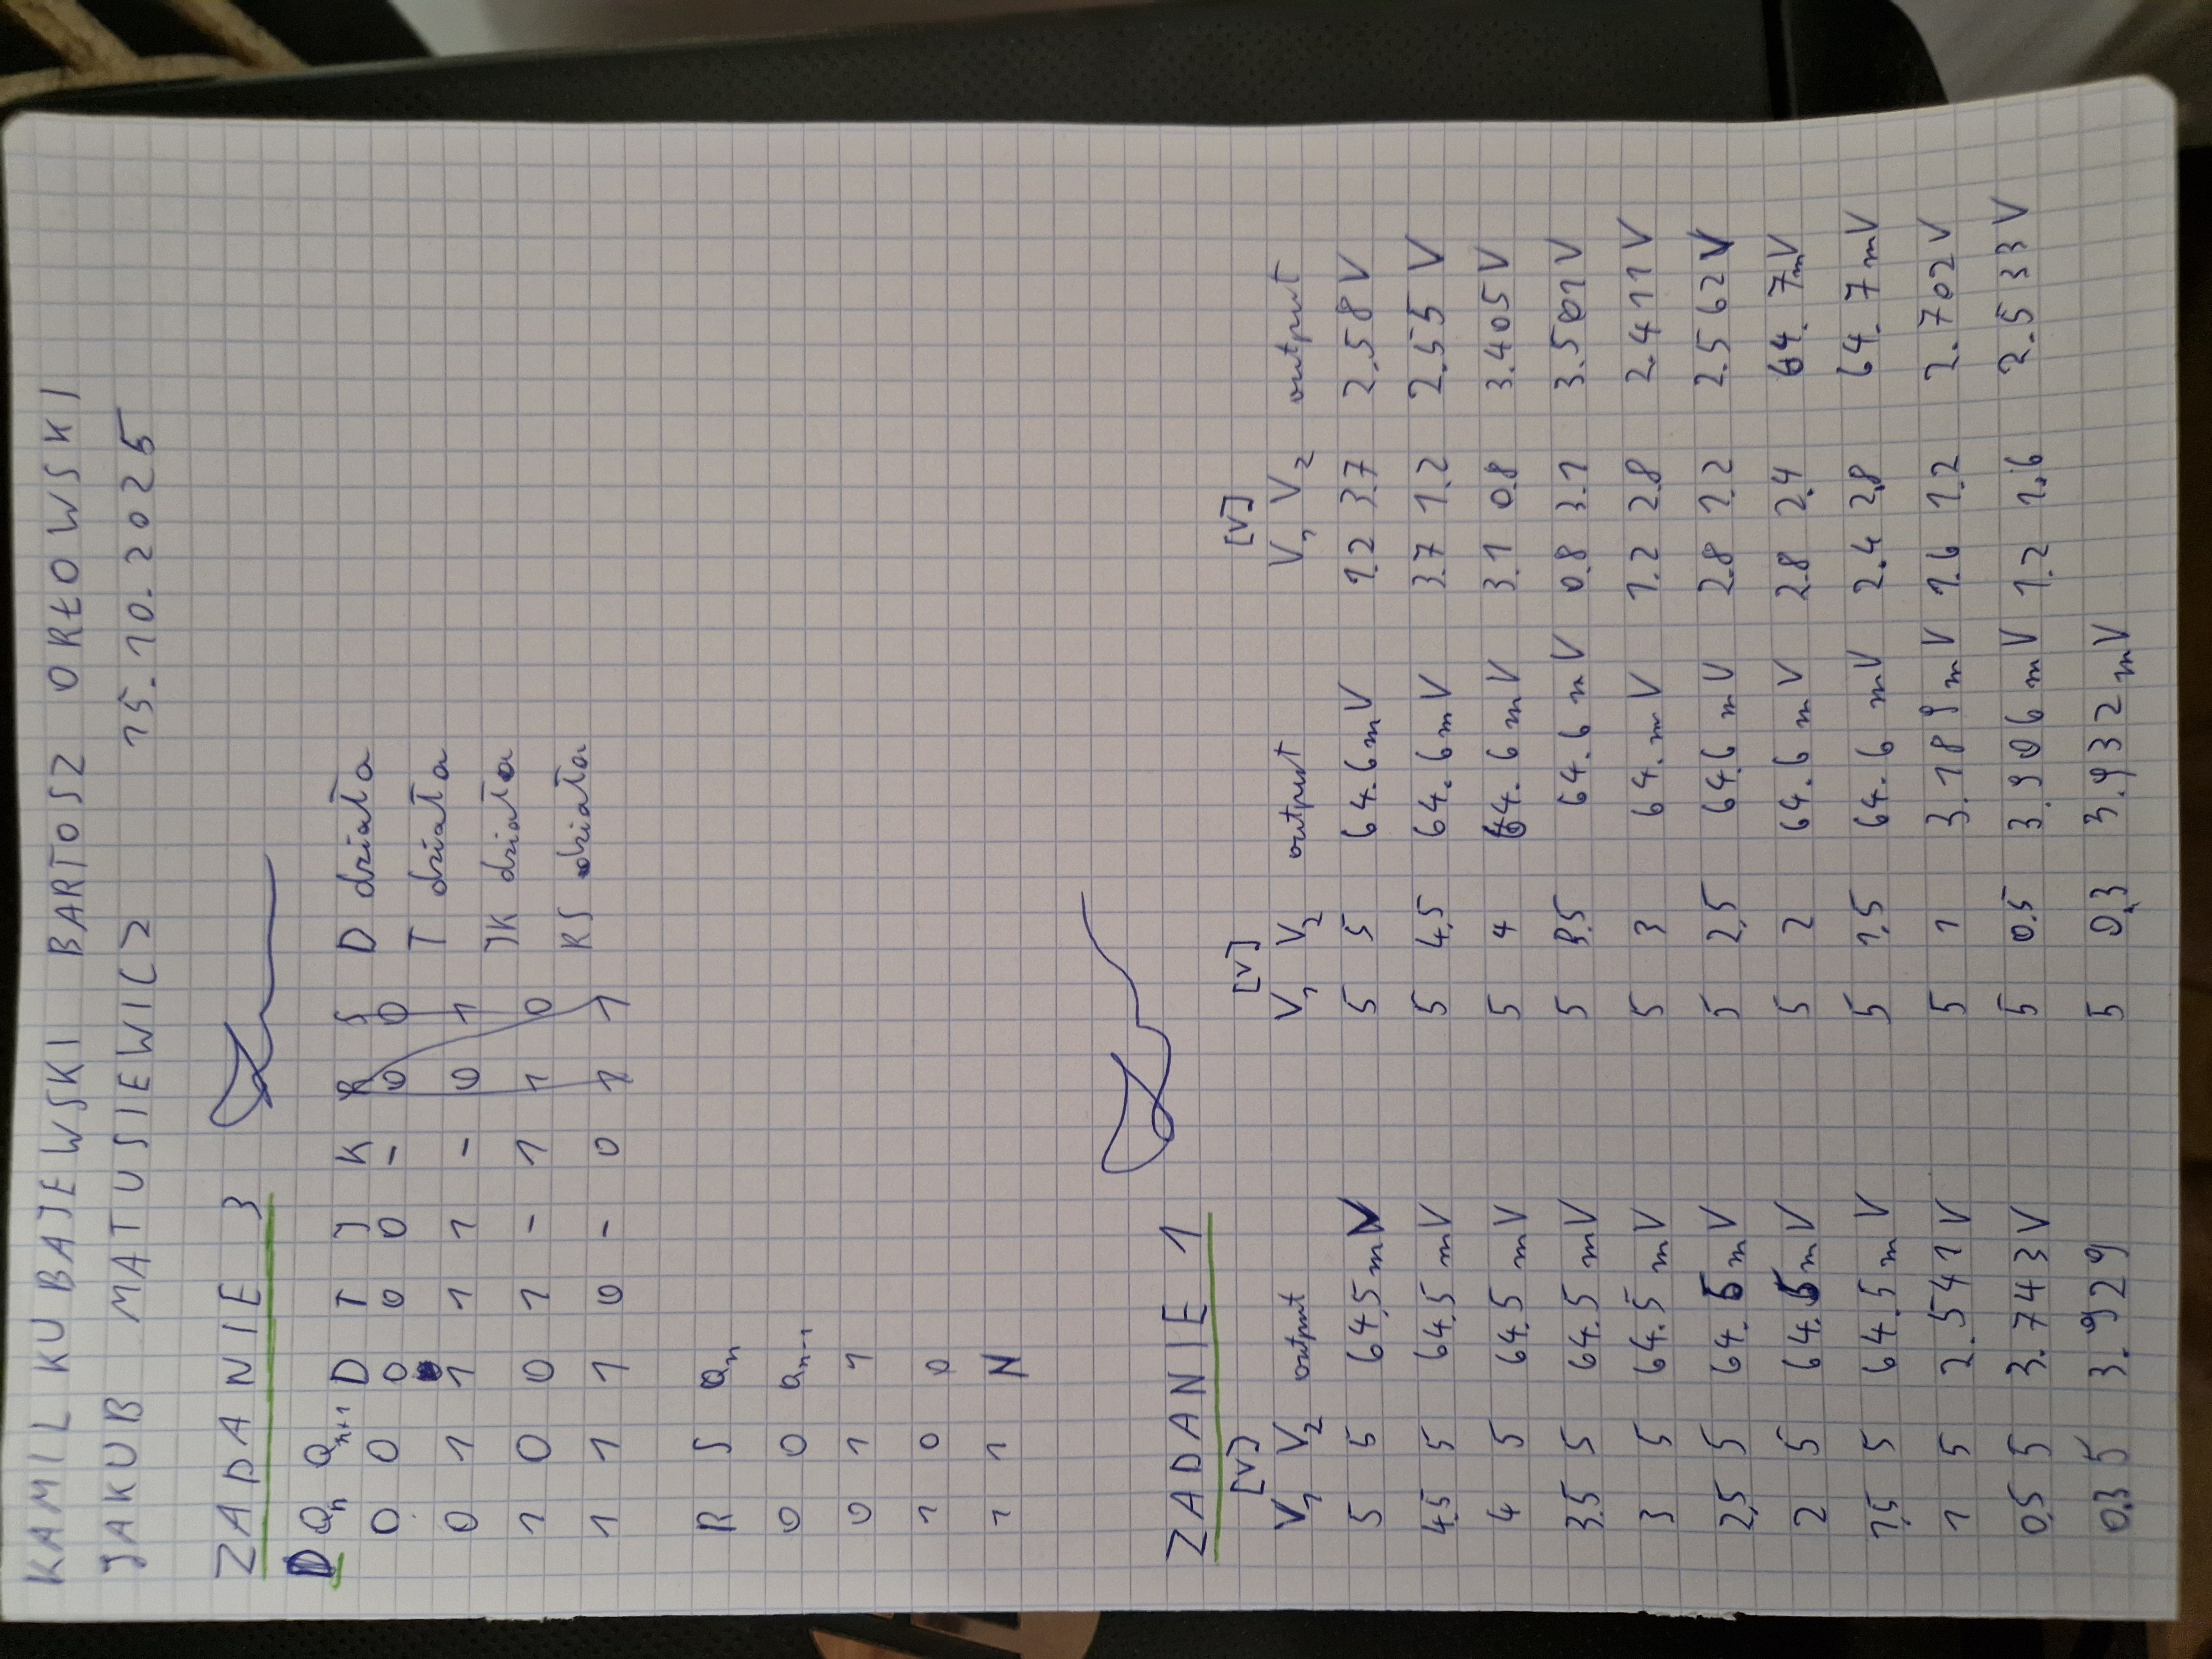
\includegraphics[width=0.8\textwidth, angle=-90]{protokol.JPG}
    \caption{Protokół}
    \label{fig:moj_obrazek}
\end{figure}
\end{document}